\section{Related Work}

\subsection{Deep Q-Networks}

The work of Mnih et al. \cite{mnih2013playingatarideepreinforcement} led to the implementation of DQNs that successfully played Atari 2600 games, outperforming human experts in several games. The DQN architecture integrates a convolutional neural network (CNN) to approximate Q-values, and uses experience replay to reduce data correlation and stabilize the learning process. This methodology has been shown to be robust and effective, and has formed the basis for many subsequent studies in the field. A detailed explanation of how DQNs work, including the architecture and training process, is provided in subsection \ref{subsec: DQN}.

\subsection{Double DQN}
Several extensions of the original DQN algorithm have been developed to further improve its performance and stability. Double DQN, introduced by Van Hasselt et al. \cite{van_Hasselt_Guez_Silver_2016}, aims to reduce Q-value overestimation by using two separate networks, one for action selection and another for Q-value calculation.
%vorstellen in kapitel x.

\subsection{Experience Replay}
% Not uses in our paper
%Another notable extension is the Dueling DQN by Wang et al. \cite{pmlr-v48-wangf16}, which decomposes the Q-value function into two separate estimates: one for the benefit of a given action and another for the value of the state. This separation allows the agent to better evaluate the relative quality of actions in a given state, leading to faster and more stable learning.


%also not used in our paper, we use "normal distribution" experience replay
%\subsection{Prioritized Experience Replay}
%Schaul et al. \cite{schaul2016prioritizedexperiencereplay} introduced the concept of prioritised experience replay, where experiences are sampled based on their importance to learning rather than randomly. This technique improves training efficiency by ensuring that experiences that are more important and informative are replayed more often. 


% not relevant to our paper in my opinion
\begin{comment}
\subsection{Hierarchical Reinforcement Learning}
Another approach to enhancing the efficiency and scalability of RL is Hierarchical Reinforcement Learning (HRL). Dietterich \cite{dietterich2000hierarchical} introduced the MAXQ framework, which decomposes the learning task into a hierarchy of subtasks. This hierarchy helps the agent tackle complex tasks by breaking down the learning objectives into more manageable steps.
\end{comment}

\section{Contributions}
This paper extends the work of Mnih et al. \cite{mnih2013playingatarideepreinforcement} by implementing Double Deep Q-Networks (Double DQN) by Van Hasselt et al. \cite{van_Hasselt_Guez_Silver_2016}, which utilizes two separate networks for action selection and Q-value estimation. We then provide detailed analysis and insights into the training process, challenges encountered, and potential improvements.

\section{Atari Video Pinball Game}

\begin{figure}[!h]
\centering
\centerline{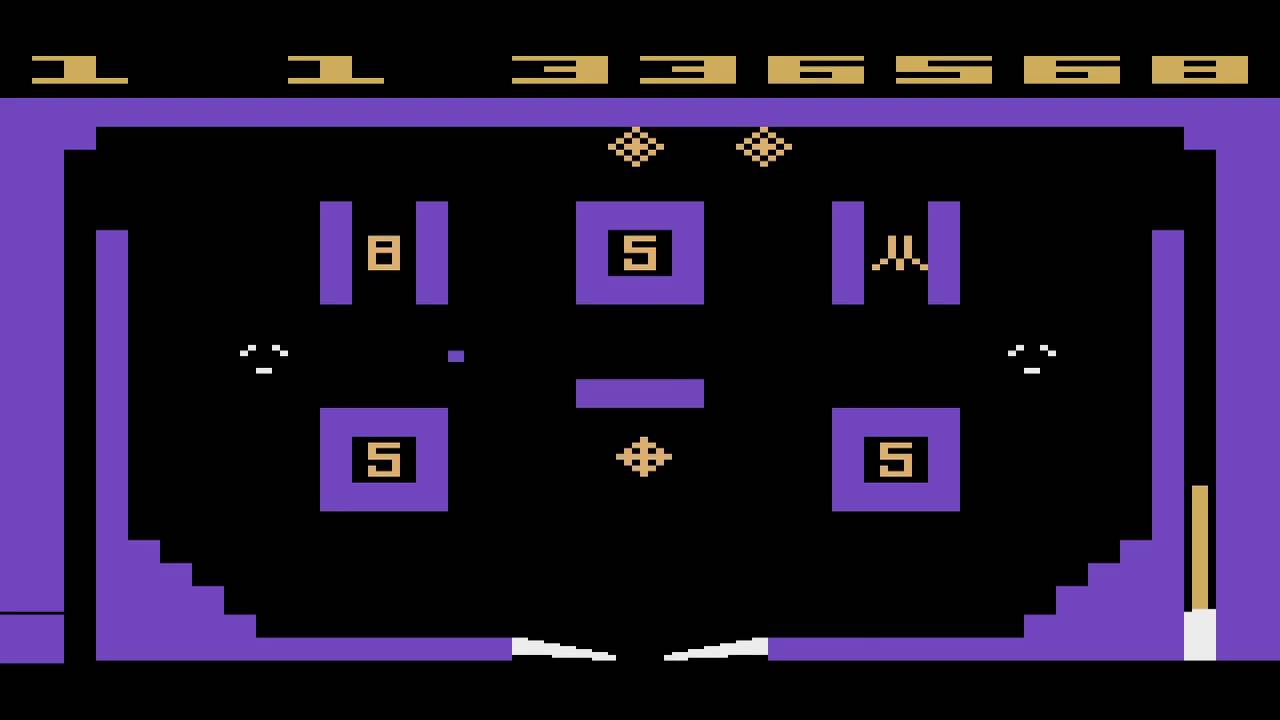
\includegraphics[scale=0.17]{graphics/game.jpg}}
\caption{This figure presents a demo of the actual game.}
\label{fig: game}
\end{figure}

"Atari Video Pinball", released by Atari, Inc. in 1980 for the Atari VCS (later known as the Atari 2600), is a video game that simulates the experience of playing a pinball machine. The game was developed by Bob Smith and incorporates essential elements of pinball, including flippers, bumpers, and a ball launcher. The player controls the aforementioned elements using the Atari joystick, thereby replicating the physical actions involved in traditional pinball gameplay. The movement of the joystick allows for the activation of the left and right flippers, while a downward pull on the joystick emulates the action of pulling back a plunger to launch the ball into play. \cite{newman2018atari}

The game is designed to emulate the dynamics of an arcade pinball machine, with digital enhancements. For example, the player is rewarded with an additional ball upon hitting the Atari logo on the playfield four times, thereby introducing an engaging element to the gameplay. Furthermore, the game incorporates features such as ball nudging, which enables players to subtly adjust the ball’s trajectory by holding down the joystick button and moving the controller. However, excessive nudging results in a state of tilt, which causes the ball to drain and simulates the response of a real pinball machine to excessive manipulation. \cite{newman2018atari}

Points are scored as follows: \cite{atari_videopinball}
\begin{itemize}
    \item SPINNERS: 1 point each time the ball hits the spinner.
    \item BUMPER: 100 times their current value. The value inside the bumper increases every time all of the diamond-shaped drop targets are knocked down.
    \item DROP TARGETS: 100 points each time a drop target is hit.
    \item ATARI ROLLOVER: 100 points; after hitting the ATARI rollover four times, you receive an extra ball. Each time it rolls over, the bonus multiplier increases by one. Only one extra ball can be awarded with each turn. The number of ATARI rollovers hit is indicated at the bottom of the screen by one Atari symbol for each hit.
    \item LEFT ROLLOVER: 100 points each time it rolls over. Its value increases by one with each hit. When the ball drains, you receive 1000 points for each time it has rolled over, up to 4000 points.
    \item SPECIAL LIT TARGET: This target lights up for only four seconds. It is located between the two lower bumpers. Each time it is hit, the screen flashes and you score 1000 points.
\end{itemize}

The bonus multiplier is tallied at the end of a turn.

This rapid scoring is accompanied with a "whirring" sound. When you have scored one million points, the score rolls over and starts again. When this happens, you do not lose the additional 999999 points; they remain part of your score. \cite{atari_videopinball}

The goal of the game is to achieve the highest possible score by skillfully using the flippers, nudging the ball, and hitting the various targets and bumpers on the playfield to maximize point accumulation and earn extra balls. This emulates the competitive and rewarding nature of traditional pinball gameplay, encouraging players to hone their reflexes and strategic planning. \cite{atari_videopinball}

%The gameplay mechanics of Atari Video Pinball entail a single-player mode in which players alternate control of the ball in order to achieve the highest possible score. The game's visual design and scoring system were innovative for their time, offering a digital representation of the physical pinball experience. It represents a notable example of early video game design, wherein developers sought to bring popular arcade experiences into the home environment. \cite{newman2018atari}

%In conclusion, "Atari Video Pinball" represents a notable early instance of video gaming that effectively translated the excitement and challenge of pinball into a home console format. The innovative use of the Atari joystick for game control and the engaging gameplay mechanics contribute to the significance of this title in the history of video gaming. \cite{newman2018atari}
